\section{Summary of the immersed boundary method}

Consider a $d$-dimensional ($d=2$ or 3) rectangular domain $\domain$, which is
filled with a viscous incompressible fluid with constant viscosity $\mu$ and
density $\rho$, and contains an immersed elastic structure, $\interface$. The
structure is impermeable to the fluid and moves at the local fluid velocity, is
deformed by this motion, and imparts a force on the fluid. Otherwise, the
interface is treated as part of the fluid. 

The fluid velocity, $\u = \u(\x,\,t)$, is governed by the
incompressible Navier-Stokes equations for a Newtonian fluid,
\begin{gather}
    \label{eq:ins-momentum}
    \rho(\u_t + \u\cdot\grad\u) = \mu\Delta\u - \grad p + \f, \\
    \label{eq:ins-incompressibility}
    \div\u = 0,
\end{gather}
where $p$ is the hydrostatic pressure and $\f$ is the elastic force
density. This is a set of $d+1$ equations in $d+1$ unknowns: the $d$ components
of $\u$, and $p$. The equations are written relative to the Eulerian
frame, so that the coordinates $\x$ are independent variables. Quantities
in the Eulerian frame are written in the lower case Latin alphabet.

Let $\X=\X(\params,\,t)$ represent a parametrization of the
Cartesian coordinates of an immersed interface with material coordinates
$\params$ at time $t$. Let $\L[\X]$ be the energy density
functional for the elastic interface material. The elastic force density is
computed by evaluating the Fréchet derivative of $\L$,
\begin{equation}
    \F = -\delta \L[\X],
\end{equation}
where $\delta$ represents the first variation. Upper case Latin letters
represent Lagrangian quantities and are functions of $\params$ and $t$.

To couple the fluid and interface, we employ the Dirac delta function,
$\Dirac(\x-\X(\params,\,t))$. Analytically, the fluid-interface
interactions can be written
\begin{gather}
    \label{eq:interpolation}
    \U = \int_\domain \Dirac(\x-\X) \u(\x,\,t)\d\x,\ \text{and} \\
    \label{eq:spreading}
    \f = \int_\interface \Dirac(\x-\X)\F(\X)\d\X,
\end{gather}
where $\U$ represents the derivative of $\X$ with respect to $t$.
[Equation @eq:interpolation] is called interpolation, and the result of the
right-hand side is the fluid velocity at $\X$; namely, $\U = \u(\X,\,t)$.
[Equation @eq:spreading] is called spreading, because while $\F$ has units of
force per unit \emph{area} on $\interface$, $\f$ has units of force per unit
\emph{volume} in $\domain$. The force $\F\d\X$ over area $\d\X$ is ``spread''
to the force $\f\d\x$ over volume $\d\x$. 

Each of the fluid equations is discretized on a regular grid of spacing $h$ so
that $\domain$ is divided into cubic cells of side length $h$. The grids can be
collocated or staggered. Because of the checkerboard instability (see, e.g.,
[@Wesseling:2001ci]) in solving the Navier-Stokes equations on collocated
regular grids, we will assume that the grids are staggered. This means that
different components of a single Eulerian vector quantity, such as $\u$,
might be evaluated at different locations. However, corresponding components of
vector-valued Eulerian quantities, and those of $\u$ and $\f$ in
particular, are assumed to be discretized on the same grid. A fixed Lagrangian
point may reside in different grid cells for each different grid. The set of
Eulerian grid points for a grid will be denoted $\domain^h$, and define
$n_\omega = |\domain^h|$.

The Lagrangian force density $\F$ is evaluated at a set of points, usually a
\emph{fixed} set of points in the Lagrangian variables, $\vec{\theta}$. The
notation $\X_j=\X(\params_j,\,t)$ refers to an individual Lagrangian point. The
typical heuristic for distributing the points $\X_j$ on the elastic interface
is that neighboring Lagrangian points be at most $h$ apart from one another,
and often at most $h/2$ apart. We denote the set of Lagrangian points by
$\interface^h$ and define $n_\gamma = |\interface^h|$ to be the number of
Lagrangian points.

\begin{figure}[thb]
    \centering
    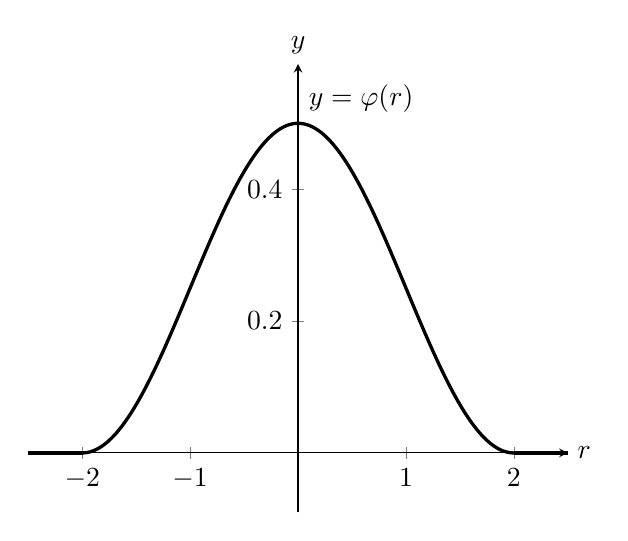
\begin{tikzpicture}
        \begin{axis}[ymin=-0.09, ymax=0.59, xmin=-2.5, xmax=2.5, axis lines=center, xlabel={$r$}, ylabel={$y$}, xlabel style={right}, ylabel style={above}, smooth, no markers]
            \addplot[samples=400, domain=-2: 2, very thick, black] {0.25 * (1+cos(90*x))} node[midway, above right] {$y=\varphi(r)$};
            \addplot[samples=400, domain=-3:-2, very thick, black] {0};
            \addplot[samples=400, domain= 2: 3, very thick, black] {0};
        \end{axis}
    \end{tikzpicture}
    \caption{%
        A compactly-supported approximation to the Dirac delta function. The
        quantity $r$ is the difference in position of an Eulerian and
        a Lagrangian point in units of grid spaces. For $r\in[0,\,1)$, only
        $\varphi(r-2)$, $\varphi(r-1)$, $\varphi(r)$, and $\varphi(r+1)$ are
        nonzero for points spaced 1 apart.
    }
    \label{fig:1d-kernel}
\end{figure}

The singular [integrals @eq:interpolation;@eq:spreading] do not lend themselves
easily to evaluation. In particular, it is unlikely that Lagrangian points and
Eulerian grid points will coincide. For a regular grid with spacing $h$, we
replace the Dirac $\Dirac$-function with a regularized kernel, $\Dirac_h$,
which is a Cartesian product of one-dimensional kernels,
$h^{-1}\kernel(h^{-1}x)$. One choice for $\kernel$ is shown in
[@fig:1d-kernel]. 

A single step of the IB method proceeds roughly as follows:
\begin{enumerate}[label=(\texttt{\alph*})]
    \item interpolate $\u^n$ to $\X^n$ to get $\vec{U}^\ast$,
    \item predict data site positions $\X^\ast = \X^n + \alpha k\U^\ast$,
    \item compute Lagrangian forces $\F^\ast$ using positions $\X^\ast$,
    \item spread $\F^\ast$ from $\X^\ast$ to get $\f^\ast$,
    \item solve for updated velocities $\u^\ast$,
    \item project $\u^\ast$ into space of divergence-free vector fields to
        get $\u^{n+1}$,
    \item interpolate $\u^{n}$ to $\X^n$ to get $\vec{U}^{n+1}$, and
    \item update $\X^{n+1} = \X + k \U^{n+1}$.
\end{enumerate}
We group these steps into 3 categories: the purely Eulerian
(\texttt{e}) and (\texttt{f}); the purely Lagrangian (\texttt{b}), (\texttt{c}),
and (\texttt{h}); and the Euler-Lagrange coupling (\texttt{a}), (\texttt{d}),
and (\texttt{g}). The description of the methods are divided according to these
categories
